\section{Punto de Vista de Cooperación de Aplicación}

El punto de vista de la cooperación de aplicaciones describe las relaciones entre los componentes de las aplicaciones en términos de los flujos de información entre ellos, o en términos de los servicios que ofrecen y utilizan. Este punto de vista se utiliza normalmente para crear una descripción general del panorama de aplicaciones de una organización. Este punto de vista también se utiliza para expresar la cooperación (interna) u orquestación de servicios que, en conjunto, apoyan la ejecución de un proceso empresarial.

\subsection{Modelo de Cooperación de Aplicación}
\begin{figure}[h!]
	\centering
	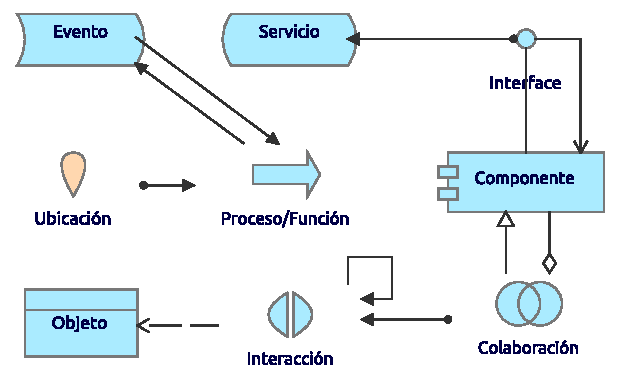
\includegraphics[width=.8\linewidth]{imgs/modelo/CoopAplicacion}
	\caption{Modelo Cooperación de Aplicación}
\end{figure}

El punto de vista de cooperación de aplicación de la capa de aplicación consta de una gran serie de elementos que se articulan entre ellos para dar a conocer los componentes del proyecto y la relación existente entre ellos. Entre los componentes de este punto de vista se encuentra la ubicación, el evento, la interacción, el proceso que cumple y como principal el componente con su interfaz y servicio.

\newpage

\subsection{Caso  de Cooperación de Aplicación}
\begin{figure}[h!]
	\centering
	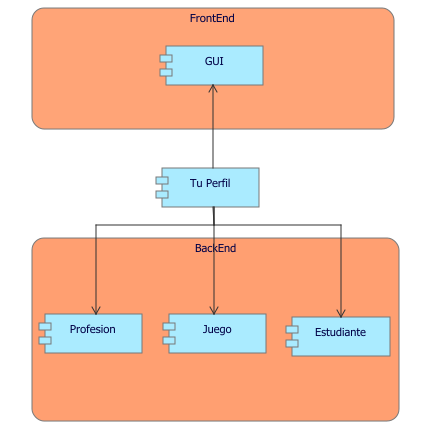
\includegraphics[width=.8\linewidth]{imgs/caso/aplicacion/CoopAplicacion}
	\caption{Caso Cooperación de Aplicación}
\end{figure}

En el caso del proyecto "Tu Perfil" y para el punto de vista de cooperación de aplicación, se cuenta con un componente principal, el cual es el que hace las veces de orquestador, en la parte del back se ubican tres componentes que en su orden estricto son: en primer lugar el componente contexto, el cual da la aplicabilidad al juego, es decir, selección u orientación para la escogencia del juego, como aplica al juego para su perfilamiento; el juego con su interfaz de jugabilidad; el perfilamiento que es como dar un resultado de acuerdo al juego para perfilar al usuario y el estudiante, el que tiene la interacción o comunicación con el orquestador para acceder a realizar un perfilamiento.

\newpage